\documentclass[aspectratio=169]{beamer}
\usepackage{will_handley}

% Commands
% --------
% - \arxiv{arxiv number}
% - \cols{width}{lh column}{rh column}
% -  \begin{fig(left|right)}[fractional width (e.g 0.6) ]{name of image}
%        content of other column
%    \end{fig(left|right)}

% Talk details
% ------------
\title{Next generation cosmological analysis with nested sampling}
\date{8\textsuperscript{th} September 2022}
\newcommand{\av}[2][]{\left\langle #2\right\rangle_{#1}}

\begin{document}

\begin{frame}
    \titlepage
\end{frame}

\begin{frame}
    \frametitle{Overview}
    \begin{columns}
        \column{0.5\textwidth}
        \begin{itemize}
            \item DiRAC 2020 RAC allocation of 30MCPUh
            \item Main goal: Planck Legacy Archive equivalent
            \item Parameter estimation $\to$ Model comparison
            \item MCMC $\to$ Nested sampling
            \item Planck $\to$ $\{\text{Planck}, \text{DESY1}, \text{BAO}, \ldots \}$
            \item Pairwise combinations
            \item Suite of tools for processing these 
                \begin{itemize}
                    \item \texttt{anesthetic} $2.0$
                    \item \texttt{unimpeded} $1.0$
                    \item \texttt{zenodo} archive
                \end{itemize}
            \item MCMC chains also available.
            \item Work in progress, but beta testers requested (email \href{mailto:wh260@cam.ac.uk}{wh260@cam.ac.uk})
        \end{itemize}
        \column{0.5\textwidth}
        
\includegraphics[width=\textwidth]{logos/dirac}
        \includegraphics[width=0.5\textwidth,page=21]{figures/himmelblau}%
        \includegraphics[width=0.5\textwidth,page=15]{figures/himmelblau}
    \end{columns}
\end{frame}

\begin{frame}
    \frametitle{The three pillars of Bayesian inference}
    \begin{columns}[t]
        \column{0.33\textwidth}
        \begin{block}{Parameter estimation}
            What do the data tell us about the parameters of a model?

            \textit{e.g. the size or age of a $\Lambda$CDM universe}
            \[ \hspace{-10pt}\C[0]{P(\theta|D,M)} = \frac{\C[2]{P(D|\theta,M)} \C[1]{P(\theta|M)}}{\C[3]{P(D|M)}}, \] 
            \[ \C[0]{\mathcal{P}} = \frac{\C[2]{\mathcal{L}} \times\C[1]{\pi}}{\C[3]{\mathcal{Z}}}, \] 
            \[ \C[0]{\text{Posterior}} = \frac{\C[2]{\text{Likelihood}} \times\C[1]{\text{Prior}}}{\C[3]{\text{Evidence}}}. \]
        \end{block}
        \column{0.33\textwidth}
        \begin{block}{Model comparison}
            How much does the data support a particular model?

            \textit{e.g. $\Lambda$CDM vs a dynamic dark energy cosmology}
            \[ \C[4]{P(M|D)} = \frac{\C[3]{P(D|M)} \C[5]{P(M)}}{\C[6]{P(D)}}, \] \[ \frac{\C[3]{\mathcal{Z}_\mathcal{M}} \C[5]{\Pi_\mathcal{M}}}{\C[6]{\sum_m Z_m \Pi_m}}, \] \[ \C[4]{\text{Posterior}} = \frac{\C[3]{\text{Evidence}} \times\C[5]{\text{Prior}}}{\C[6]{\text{Normalisation}}}.\]
        \end{block}
        \column{0.33\textwidth}
        \begin{block}{Tension quantification}
            Do different datasets make consistent predictions from the same model? 

            \textit{e.g. CMB vs Type IA supernovae data}
            \[ \mathcal{R} = \frac{\mathcal{Z}_{AB}}{\mathcal{Z}_A\mathcal{Z}_\mathcal{B}}, \] 
            \[
                \begin{aligned} \log\mathcal{S} = \av[\mathcal{P}_{AB}]{\log\mathcal{L}_{AB}}&\\
                    -\av[\mathcal{P}_{A}]{\log\mathcal{L}_{B}}&\\
                    -\av[\mathcal{P}_{B}]{\log\mathcal{L}_{B}}&
                \end{aligned}
            \]
        \end{block}
    \end{columns}
\end{frame}

\begin{frame}
    \frametitle{Occam's Razor~\arxiv{2102.11511}}
    \begin{itemize}
        \item Bayesian inference quantifies Occam's Razor:
            \begin{itemize}
                \item \textit{``Entities are not to be multiplied without necessity''} \hfill --- William of Occam
                \item \textit{``Everything should be kept as simple as possible, but not simpler''} \hfill --- ``Albert Einstein''
            \end{itemize}
        %\item Consider the Evidence $\C[3]{\mathcal{Z}\equiv P(D|M)}$: 
        %    \begin{description}[Parameter estimation]
        %        \item [Parameter estimation] normalisation constant
        %        \item [Model comparison] critical update factor for \C[5]{model prior} to \C[4]{model posterior}
        %    \end{description}
        \item Properties of the evidence: rearrange Bayes' theorem for parameter estimation
            \[\C[0]{\mathcal{P}(\theta)} = \frac{\C[2]{\mathcal{L}(\theta)} \C[1]{\pi(\theta)}}{\C[3]{\mathcal{Z}}} \qquad\Rightarrow\qquad \C[3]{\log \mathcal{Z}} = \C[2]{\log\mathcal{L}(\theta)} - \log \frac{\C[0]{\mathcal{P}(\theta)}}{\C[1]{\pi(\theta)}} \]  
        \item Evidence is composed of a ``goodness of fit'' term  and ``Occam Penalty''
    \end{itemize}
    \begin{columns}[t]
        \column{0.5\textwidth}
        \begin{itemize}
            \item RHS true for all $\theta$. Take max likelihood value $\theta_*$:
                \[
                    \C[3]{\log \mathcal{Z}} = -\chi_\mathrm{min}^2 - \text{Mackay penalty}
                \]
        \end{itemize}
        \column{0.5\textwidth}
        \begin{itemize}
            \item Be more Bayesian and take posterior average to get the ``Occam's razor equation''
                \[
                    \boxed{
                        \C[3]{\log \mathcal{Z}} = \av[{\C[0]{\mathcal{P}}}]{\C[2]{\log\mathcal{L}}} - \mathcal{D}_\mathrm{KL}
                    }
                \]
        \end{itemize}
    \end{columns}
    \vfill
    \begin{itemize}
        \item Natural regularisation which penalises models with too many parameters.
    \end{itemize}
\end{frame}

\begin{frame}
    \frametitle{Kullback Liebler divergence}
    \begin{columns}
        \column{0.5\textwidth}
        \begin{itemize}
            \item The KL divergence between \C[1]{prior $\pi$} and \C[0]{posterior $\mathcal{P}$} is is defined as:
                \[\mathcal{D}_\mathrm{KL} = \av[\mathcal{P}]{\log\frac{\mathcal{P}}{\pi}} = \int \mathcal{P}(\theta) \log \frac{\mathcal{P}(\theta)}{\pi(\theta)}d\theta.\]
            \item Whilst not a distance, $\mathcal{D}=0$ when $\mathcal{P}=\pi$.
            \item Occurs in the context of machine learning as an objective function for training functions.
            \item In Bayesian inference it can be understood as a log-ratio of ``volumes'':
                \[ \mathcal{D}_\mathrm{KL} \approx \log \frac{V_\pi}{V_\mathrm{P}}.\]
                (this is exact for top-hat distributions).
        \end{itemize}
        \column{0.5\textwidth}
        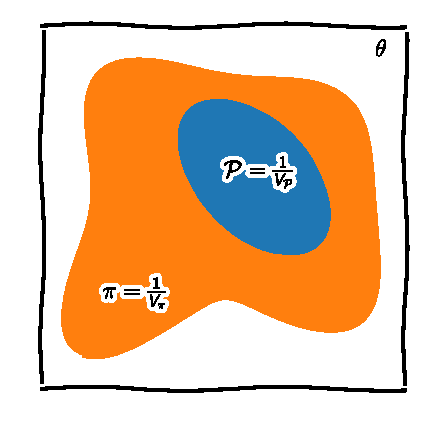
\includegraphics{figures/volumes.pdf}
    \end{columns}
\end{frame}

\begin{frame}
    \frametitle{Why do sampling?}
    \begin{columns}
        \column{0.5\textwidth}
        \begin{itemize}
            \item The cornerstone of numerical Bayesian inference is working with \C[3]{samples}.
            \item Generate a set of representative parameters drawn in proportion to the posterior $\theta\sim\mathcal{P}$.
            \item The magic of marginalisation $\Rightarrow$ perform usual analysis on each sample in turn.
            \item The golden rule is \C[1]{stay in samples} until the last moment before computing summary statistics/triangle plots because \[\boxed{f(\:\av{X}\:)\ne \av{\:f(X)\:}}\]
            \item Generally need $\sim\mathcal{O}(12)$ independent samples to compute a value and error bar.
        \end{itemize}
        \column{0.5\textwidth}
        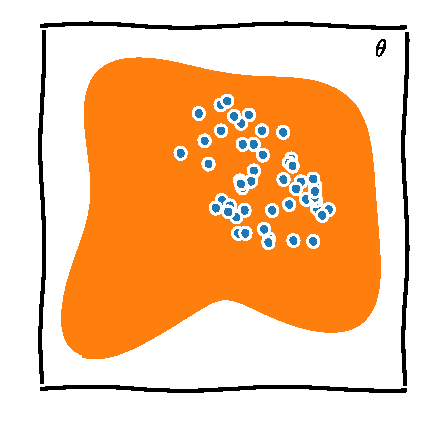
\includegraphics{figures/samples.pdf}
    \end{columns}
\end{frame}

\begin{frame}
    \frametitle{The Planck legacy archive}
    \begin{columns}
        \column{0.5\textwidth}
        \begin{itemize}
            \item \textit{Planck} collaboration science products
            \item distributed cosmology inference results as MCMC chains
            \item Across a grid of:
                \begin{itemize}
                    \item subsets/combinations of \textit{Planck} data
                        \begin{itemize}
                            \item TT, lowl, lowE, lensing
                        \end{itemize}
                    \item $\Lambda$CDM extensions 
                        \begin{itemize}
                            \item base, mnu, nrun, omegak, r
                        \end{itemize}
                \end{itemize}
            \item importance sampling across some other likelihoods (BAO, JLA,\ldots)
            \item Cannot compute evidences in high dimensions from MCMC chains
                \begin{itemize}
                    \item Only parameter estimation
                    \item no model comparison
                \end{itemize}
        \end{itemize}
        \column{0.5\textwidth}
        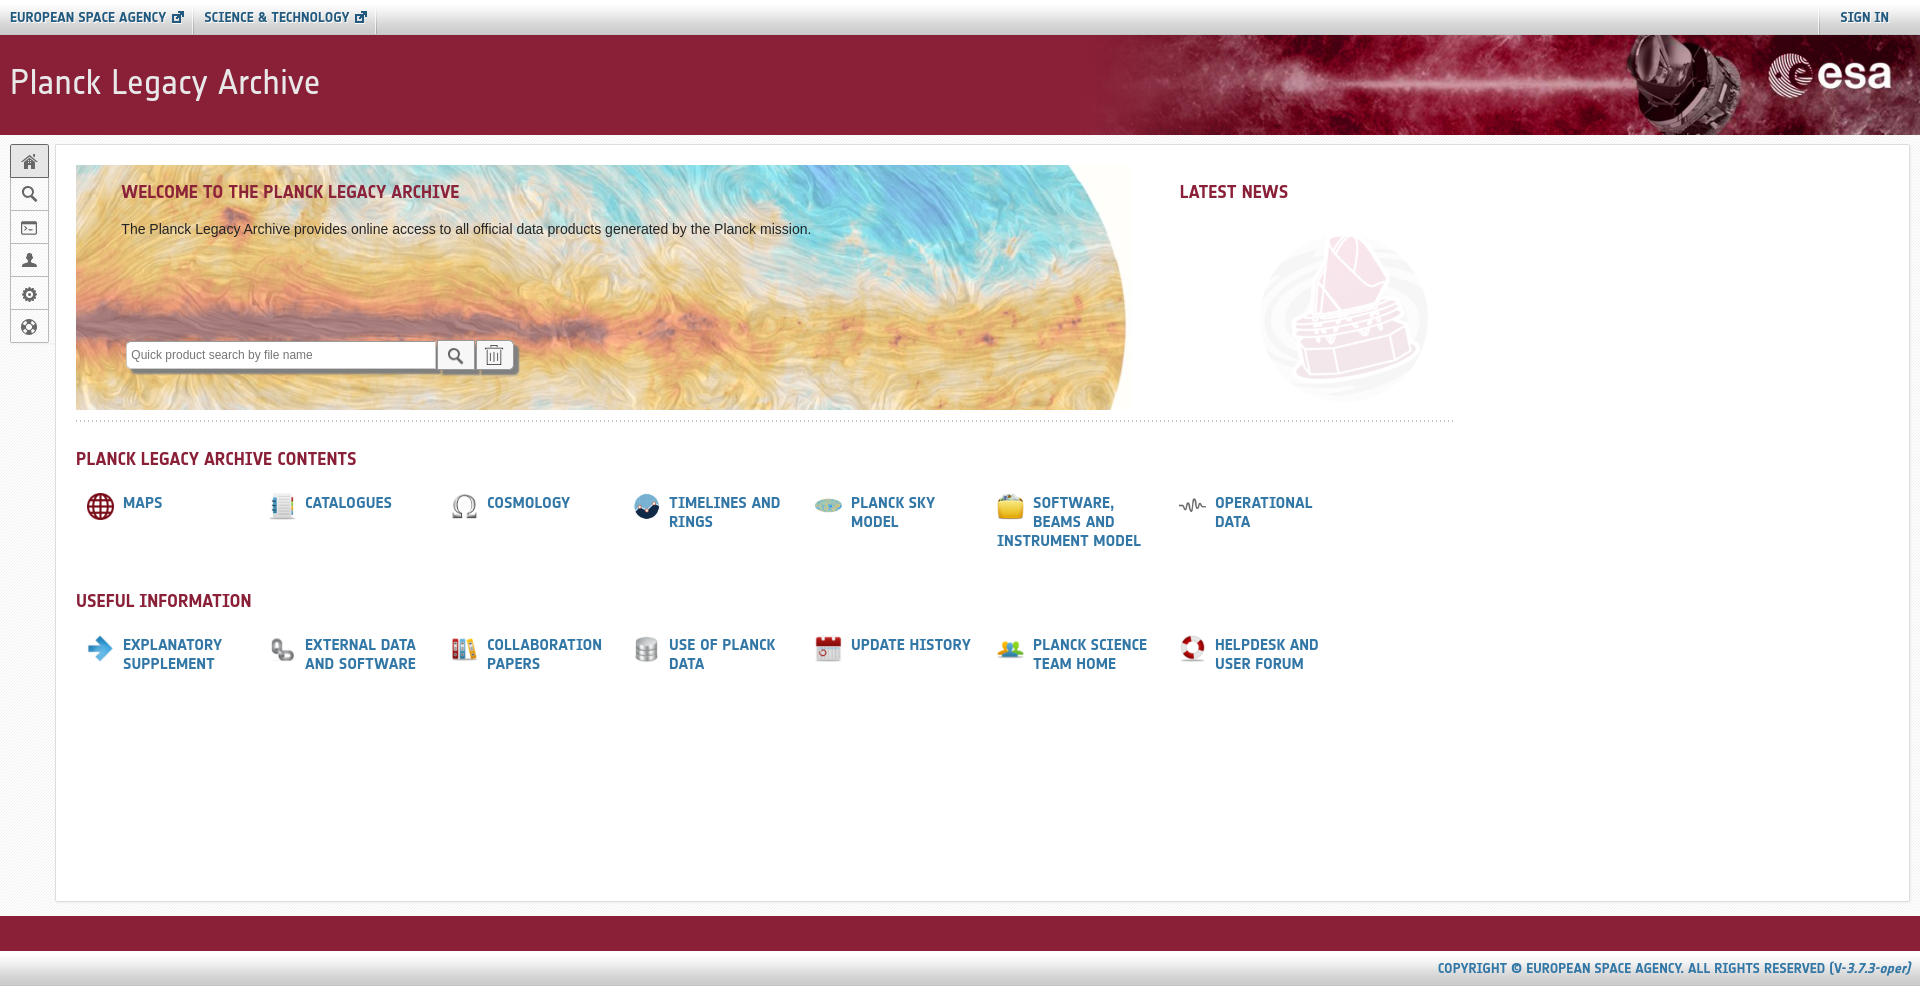
\includegraphics[width=\textwidth]{figures/pla}
        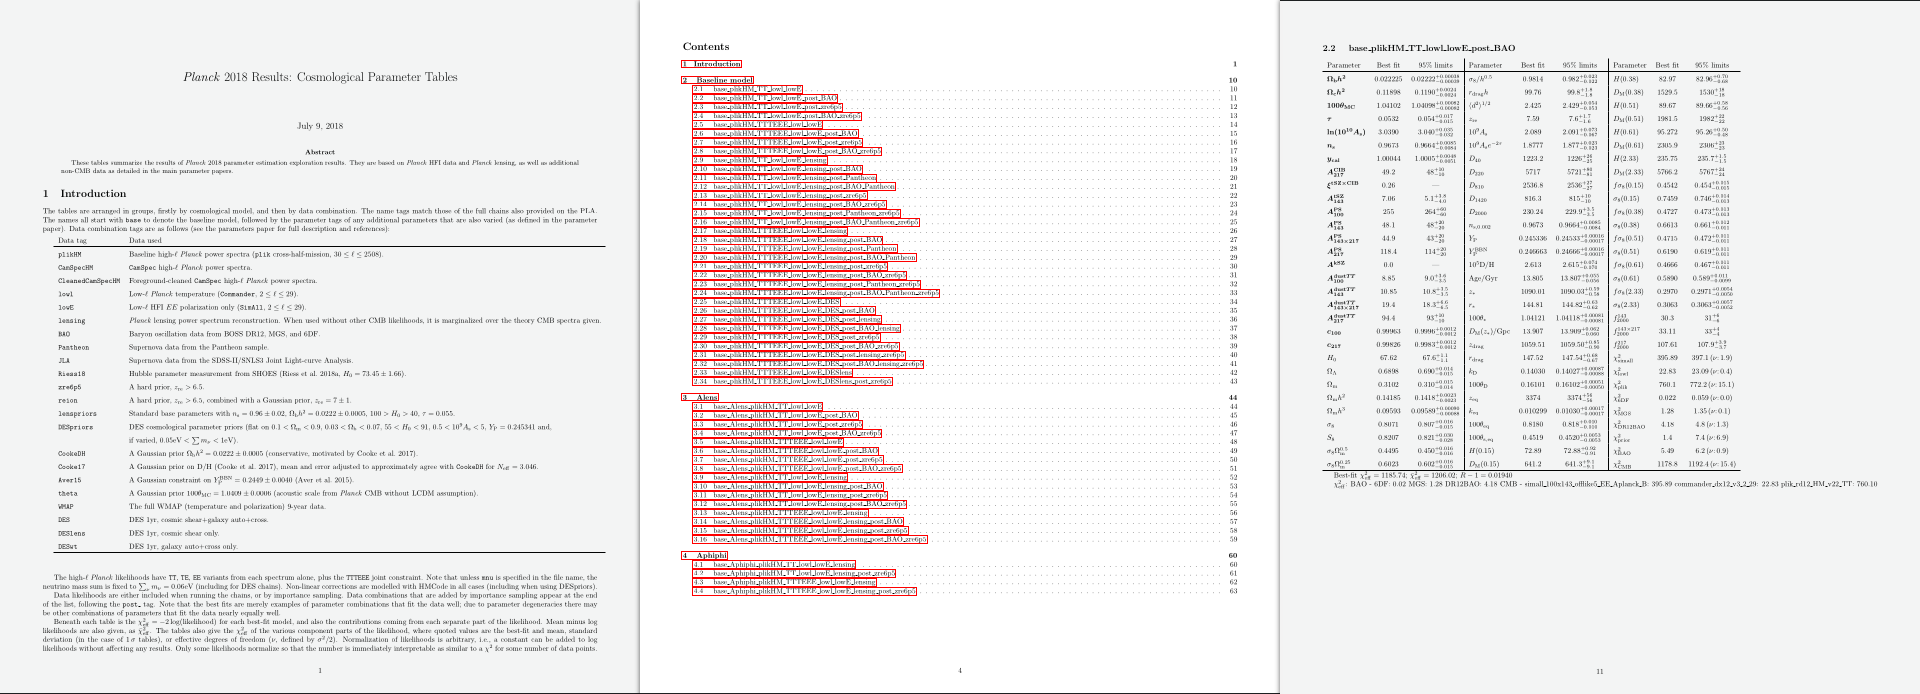
\includegraphics[width=\textwidth]{figures/pla1}
    \end{columns}
\end{frame}

\begin{frame}
    \begin{columns}
        \column{0.5\textwidth}
        \begin{block}{\textbf{MCMC}}
            \includegraphics<1>[width=\textwidth,page=16]{figures/himmelblau}%
            \includegraphics<2>[width=\textwidth,page=17]{figures/himmelblau}%
            \includegraphics<3>[width=\textwidth,page=18]{figures/himmelblau}%
            \includegraphics<4>[width=\textwidth,page=19]{figures/himmelblau}%
            \includegraphics<5>[width=\textwidth,page=20]{figures/himmelblau}%
            \includegraphics<6-15>[width=\textwidth,page=21]{figures/himmelblau}%
            \begin{itemize}
                \item<16> Single ``walker''
                \item<16> Explores posterior
                \item<16> Fast, if proposal matrix is tuned
                \item<16> Parameter estimation, suspiciousness calculation
                \item<16> Channel capacity optimised for generating posterior samples
            \end{itemize}
        \end{block}
        \centerline{\includegraphics<16>[width=0.5\textwidth,page=19]{figures/himmelblau}}
        \column{0.5\textwidth}
        \begin{block}<7->{\textbf{Nested sampling}}
            \includegraphics<7|handout:0>[width=\textwidth,page=1]{figures/himmelblau}%
            \includegraphics<8|handout:0>[width=\textwidth,page=2]{figures/himmelblau}%
            \includegraphics<9|handout:0>[width=\textwidth,page=3]{figures/himmelblau}%
            \includegraphics<10          >[width=\textwidth,page=4]{figures/himmelblau}%
            \includegraphics<11|handout:0>[width=\textwidth,page=5]{figures/himmelblau}%
            \includegraphics<12|handout:0>[width=\textwidth,page=6]{figures/himmelblau}%
            \includegraphics<13|handout:0>[width=\textwidth,page=7]{figures/himmelblau}%
            \includegraphics<14|handout:0>[width=\textwidth,page=8]{figures/himmelblau}%
            \includegraphics<15|handout:0>[width=\textwidth,page=15]{figures/himmelblau}%
            \begin{itemize}
                \item<16> Ensemble of ``live points''
                \item<16> Scans from prior to peak of likelihood
                \item<16> Slower, no tuning required
                \item<16> Parameter estimation, model comparison, tension quantification
                \item<16> Channel capacity optimised for computing partition function
            \end{itemize}
        \centerline{\includegraphics<16>[width=0.5\textwidth,page=4]{figures/himmelblau}} \end{block}
    \end{columns}
\end{frame}

\begin{frame}
    \frametitle{The grid (so far)}
    \begin{itemize}
        \item Models: $[\Lambda\text{CDM}, \Omega_K, \nu, r, w, w(a)]$
        \item Data: [\texttt{plik}, \texttt{camspec}, \texttt{DESY1}, \texttt{bicep+keck}, \texttt{BAO(DR16)}, \texttt{pantheon} ]
        \item Pairwise combinations of datasets
        \item Breakdown of Planck \& BAO data
        \item These exhaust what is currently available by default in $\texttt{cobaya}$
        \item Wide priors to allow for importance readjustment as desired
        \item roughly halfway through computational allocation. 
        \item Feedback desirable as to what extensions to the gred would be of community interest.
        \item Further checking needed before first release by end of this year.
    \end{itemize}
\end{frame}

\begin{frame}
    \frametitle{\texttt{unimpeded}}
    \framesubtitle{Universal Model comparison and Parameter Estimation Distributed over Every Dataset}
    \begin{itemize}
        \item Python tool for seamlessly downloading and cacheing chains
        \item Data stored on \texttt{zenodo} 
        \item hdf5 storage for fast \& reliable download \& storage
        \item Library of trained bijectors to be used as priors/emulators~\arxiv{2102.12478}/nuisance marginalised likelihoods~\arxiv{2207.11457}
        \item \texttt{anesthetic} compatible for processing of chains~\arxiv{1905.04768}
        \item $\alpha$-testers wanted! (email \href{mailto:wh260@cam.ac.uk}{wh260@cam.ac.uk}) 
        \item End goal -- community library which everyone contributes to so expensive runs reusable.
    \end{itemize}
\end{frame}

\begin{frame}
    \frametitle{The importance of global measures of tension}
    \begin{columns}
        \begin{column}{0.5\textwidth}
            \begin{itemize}
                \item Hubble tension~\arxiv{1907.10625}
                    \begin{itemize}
                        \item \textit{Planck}: $H_0=67.4\pm0.5$
                        \item S$H_0$ES: $H_0=74.0\pm1.4$
                    \end{itemize}
                \item In other situations the discrepancy doesn't exist in a single interpretable parameter
                \item For example: DES+\textit{Planck} \arxiv{1902.04029} 
                \item Are these two datasets in tension?
                \item There are a lot more parameters -- are we sure that tensions aren't hiding? Are we sure we've chosen the best ones to reveal the tension?
                \item Should use ``Suspiciousness'' statistic $\mathcal{S}$, or Bayes ratio $\mathcal{R}$ to determine global tension.
            \end{itemize}
        \end{column}
        \begin{column}{0.5\textwidth}
            \includegraphics<1>{figures/DES_planck_1}
            \includegraphics<2>{figures/DES_planck_2}
        \end{column}
    \end{columns}
\end{frame}


\begin{frame}
    \frametitle{The DES evidence ratio $R$}
    \begin{itemize}
        \item The Dark Energy Survey \arxiv{1708.01530} quantifies tension between two datasets $A$ and $B$ using the Bayes ratio:
            \[
                R = \frac{\mathcal{Z}_{AB}}{\mathcal{Z}_A \mathcal{Z}_B} = \frac{P(A\cap B)}{P(A)P(B)} = \frac{P(A|B)}{P(A)} = \frac{P(B|A)}{P(B)}
            \]
            where $\mathcal{Z}$ is the Bayesian evidence.
    \end{itemize}
    \begin{columns}
        \column{0.5\textwidth}
        \begin{itemize}
            \item Many attractive properties:
                \begin{itemize}
                    \item Symmetry
                    \item Parameterisation independence
                    \item Dimensional consistency
                    \item Use of well-defined Bayesian quantities
                \end{itemize}
            \item $R$ gives the relative change in our confidence in data $A$ in light of having seen $B$ (and vice-versa).
        \end{itemize}
        \column{0.5\textwidth}
        \begin{itemize}
            \item $R>1$ implies we have more confidence in $A$ having received $B$.
            \item Like evidences, it is prior-dependent \\ from $\mathcal{D}$ in $\log \mathcal{Z} = \av[\mathcal{P}]{\log\mathcal{L}}-\mathcal{D}$
            \item Increasing prior widths $\Rightarrow$ decreasing evidence. 
            \item Increasing prior widths $\Rightarrow$ increasing confidence.
        \end{itemize}
    \end{columns}
\end{frame}



\begin{frame}
    \frametitle{The DES evidence ratio $R$: Prior dependency}
    \centerline{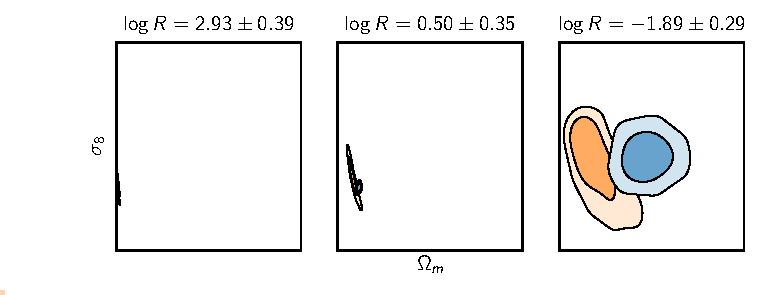
\includegraphics[trim=0.6in 0.3in 0in 0in]{./plots/prior_dependency.pdf}}
    \vspace{10pt}
    \begin{itemize}
        \item What does it mean if increasing prior widths $\Rightarrow$ increasing confidence? 
        \item Wide priors mean {\em a-priori\/} the parameters could land anywhere.
        \item We should be proportionally more reassured when they land close to one another if the priors are wide
    \end{itemize}
\end{frame}

\begin{frame}
    \frametitle{How do we deal with the prior dependency in $R$?}
    \begin{description}
        \item[Option 1] Take the Bayesian route, accept the prior dependency, and spend time trying to justify why a given set of priors are ``physical''.
        \item[Option 2] Try to find a principled way of removing this prior dependency
    \end{description}
    \begin{itemize}
        \item Decompose ratio using Occam's Razor equation $\log \mathcal{Z} = \av[\mathcal{P}]{\log\mathcal{L}} - \mathcal{D}$
        \[ 
            \begin{aligned}
                \log R &= \log\mathcal{Z}_{AB} - \log\mathcal{Z}_{A} - \log\mathcal{Z}_{A} \\
                &= \av[\mathcal{P}_{AB}]{\log\mathcal{L}_{AB}} - \av[\mathcal{P}_{A}]{\log\mathcal{L}_{A}}- \av[\mathcal{P}_{B}]{\log\mathcal{L}_{B}} - \mathcal{D}_{AB} + \mathcal{D}_{A} + \mathcal{D}_{B} \\
                &= \log \mathcal{S} + \log \mathcal{I}
            \end{aligned}
    \]
    where we have defined the suspiciousness $S$, which is prior independent, and the information $\mathcal{I}$, which depends on the parameter compression of the shared space
        \item Focussing on the prior-independent portion $\mathcal{S}$ gives $R$ for the  ``Narrowest reasonable priors'' which do not impinge on the posterior
        \item One of the critical observations is that one can only hide tension by widening priors. Narrowing them will only ever show tension if it is present.
    \end{itemize}
\end{frame}

\begin{frame}
    \frametitle{Suspiciousness $S$}
    \begin{itemize}
        \item For a Gaussian set of posteriors:
            \[
                \log \mathcal{S} = \frac{d}{2}  -\frac{1}{2} (\mu_A-\mu_B){(\Sigma_{A}+\Sigma_{B})}^{-1}(\mu_A-\mu_B).
            \]
        \item The Malhanobis  term is suggestive, so we can use this to calibrate a ``sigma'' level of tension using a $\chi^2$ distribution for $\chi^2_d=d-2\log \mathcal{S}$, or a tension probability.
        \item $S$ is composed of evidences $\mathcal{Z}$ and KL divergences $\mathcal{D}$, which are Gaussian-independent concepts, so the only thing to determine is $d$, the ``number of shared parameters''.
        \item Can do this with Gaussian dimensionality $\frac{d}{2}=\text{var}_\mathcal{P}(\log \mathcal{L})$~\arxiv{1903.06682}
            \begin{align}
                \text{Planck vs BAO}:&      &p&=  42 \pm     4 \% \nonumber\\
                \text{Planck vs DESY1}:&      &p&=   3.2 \pm     1.0 \% \nonumber\\
                \text{Planck vs S$H_0$ES}:& &p&=   0.25 \pm     0.17 \% \nonumber
            \end{align}
        \item Under this metric, S$H_0$ES is unambiguously inconsistent, although not quite as brutal as $>4\sigma$. BAO is consistent, and DESY1 is inconsistent, but only just. This is pleasingly similar to ones intuition.
    \end{itemize}

\end{frame}


\begin{frame}
    \frametitle{Curvature tension?~\arxiv{1908.09139}}

    \begin{columns}

        \begin{column}{0.5\textwidth}

            \begin{itemize}
                \item If you allow $\Omega_K\ne0$, \textit{Planck} (\texttt{plikTTTEEE}) has a moderate preference for closed universes (50:1 betting odds on), $\Omega_K=-4.5\pm1.5\%$ \hfill \arxiv{1911.02087}
                \item \textit{Planck}+lens+BAO strongly prefer $\Omega_K=0$.
                \item But, \textit{Planck} vs lensing is 2.5$\sigma$ in tension, and Planck vs BAO is 3$\sigma$.
                \item Reduced if $\texttt{plik}\to\texttt{camspec}$ \hfill\arxiv{2002.06892} 
                \item BAO and lensing summary assume $\Lambda$CDM.
                \item Doing this properly with BAO retains preference for closed universe (though closer to flat $\Omega_K =-0.4\pm0.2\%$) \hfill\arxiv{2205.05892}
                \item Present-day curvature has profound consequences for inflation \hfill\arxiv{2205.07374}
            \end{itemize}

        \end{column}

        \begin{column}{0.5\textwidth}
            \includegraphics<1|handout:0>[width=\textwidth]{figures/curvature_1}%
            \includegraphics<2|handout:0>[width=\textwidth]{figures/curvature_2}%
            \includegraphics<3          >[width=\textwidth]{figures/curvature_3}%

        \end{column}

    \end{columns}

\end{frame}

\begin{frame}
    \frametitle{Conclusions}
    \begin{itemize}
        \item DiRAC RAC allocation for building a legacy grid of
            \begin{itemize}
                \item MCMC \& Nested sampling chains
                \item gridded over (pairwise) up-to-date datasets
                \item gridded over extensions to $\Lambda$CDM
                \item Bijectors \& emulators for fast re-use
                \item Importance sampling toolkit via \texttt{anesthetic} for (re)processing
                \item Long-term goal: community repository of chains to share model comparison compute resource
            \end{itemize}
        \item Looking for:
            \begin{itemize}
                \item $\alpha$-testers for \texttt{unimpeded}
                \item Suggestions for more datasets (and their incorporation into \texttt{cobaya})
            \end{itemize}
    \end{itemize}
\end{frame}

\end{document}
